\documentclass{homework}

\title{Homework 5, Simulation}
\author{Kevin Evans}
\studentid{11571810}
\date{April 6, 2020}
\setclass{EE}{311}
\usepackage{amssymb}
\usepackage{mathtools}

\usepackage{amsthm}
\usepackage{amsmath}
\usepackage{slashed}
\usepackage{relsize}
\usepackage{threeparttable}
\usepackage{float}
\usepackage{booktabs}
\usepackage{boldline}
\usepackage{changepage}
\usepackage{physics}
\usepackage[inter-unit-product =\cdot]{siunitx}
\usepackage{setspace}

\usepackage[makeroom]{cancel}
\usepackage{pgfplots}

\usepackage{multicol}
\usepackage{tcolorbox}
\usepackage{enumitem}
\usepackage{times}
\usepackage{mhchem}
\usepackage{graphicx} 
\DeclareSIUnit{\year}{yr}

\usepackage{listings}
\lstset{basicstyle=\ttfamily,breaklines=true}

\begin{document}
	\maketitle
	The amplifier specifications are given as: \begin{itemize}
		\item Low frequency gain: exceeding $\SI{12}{\dB}$ (\SI{4}{\V/\V})
		\item Bandwidth: exceeding \SI{500}{\MHz}
		\item VDD: \SI{1.2}{\V}
	\end{itemize}
	For this circuit, the small-signal equivalent is:
	\begin{center}
		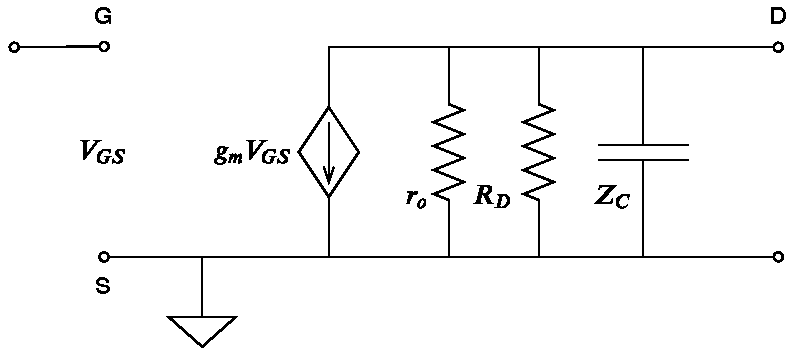
\includegraphics[width=0.7\linewidth]{acckt}
	\end{center}
	From this, the amplifier gain $G_v$ is given as \begin{align*}
		G_v & = g_m \left( r_o \parallel R_D \parallel Z_C \right) \\
			& = g_m R_{eq}
	\end{align*}
	As the capacitor has a fairly tiny value, this will be fairly neglible at lower frequencies. Nearing the bandwidth frequency, its impedance will affect the output fairly significantly, \begin{align*}
		\eval{ Z_C }_{\SI{500}{\MHz}} & = \frac{1}{j \omega C} \approx \SI{6.4}{\kohm}
	\end{align*}
	Knowing this, we must choose a drain resistance $R_D$ value that is less than $Z_C$. The transconductance and dynamic resistance is given as \begin{align*}
		g_m & = \sqrt{2 \: k_n \frac{W}{L} I_D } \\
		r_o & = \frac{1}{\lambda I_D}
	\end{align*}
	From this, we can calculate $R_D$ for any $I_D$ and aspect ratio for a target gain of 4 V/V, \begin{align*}
		R_D & = \left( R_{eq}^{-1} - r_0^{-1} \right) \\
			& = \left( \frac{g_m}{4} - r_0^{-1} \right)
	\end{align*}
	
	\pagebreak
	\noindent From the last simulation assignment (HW 2), we obtained the $I_D$-$V_{ds}$ characteristics for this NMOS transistor at its default $W/L$ ratio. From these curves, we can somewhat arbitrarily choose a bias current of $I_D = \SI{80}{\micro\ampere}$. If we use MATLAB to simply calculate the resistance, we can iterate through potential values of $W/L$ until we find a resistance $R_D$ that is near $Z_C$ at higher frequencies. 
		
\begin{lstlisting}[language=matlab]
% parameters to try out
I_d   = 80e-6;                     % drain current (A)
WL    = 32;                        % aspect ratio (um/um)

% const params, given in modelfile
Kn    = 210.88e-6;                 % (A/V^2)
L     = 1.127257;                  % lambda
Av    = 4;                         % gain (V/V)
Vtn   = 0.3074;                    % threshold voltage (V)
Vdd   = 1.2;                       % PS voltage (V)

% intermediate calculations
g_m   = sqrt(2*Kn*I_d*WL);         % transconductance
r_o   = 1 / (L*I_d);               % dynamic resistance
R_eq  = Av / g_m;                  % total output resistance

% target values
R_d   = 1/(1/R_eq - 1/r_o);        % omitting the Zc
V_ov  = sqrt(2 * I_d / (Kn * WL)); % overdrive voltage
V_g   = V_ov + Vtn;                % gate voltage
V_d   = Vdd - I_d * R_d;           % drain voltage @ I_d

disp("----------------------------------");
disp("Resistance    = " + R_d + " ohm"   );
disp("Gate voltage  = " + V_g + " V (DC)");
disp("Drain voltage = " + V_d + " V (DC)");
\end{lstlisting}
\hrule
\vspace{1em}

\noindent MATLAB output:
\begin{lstlisting}
Resistance    = 5896.5168 ohm
Gate voltage  = 0.46138 V (DC)
Drain voltage = 0.72828 V (DC)
\end{lstlisting}
	\pagebreak
	At \SI{80}{\micro\ampere}, a $W/L$ ratio of \SI{32}{\um/\um} should produce a gain of \SI{4}{\V/\V} with a drain resistance of \SI{5.9}{\kohm}, which is less than the impedance of the capacitor at the upper-bandwidth frequencies. At this bias current, the gate voltage will need to be biased at \SI{461}{\mV}. In Cadence, the circuit was built with these values: \begin{center}
		
\includegraphics[width=0.7\linewidth]{hw5_ckt}
	\end{center}
	Running the simulation, the low frequency gain is \SI{12.2}{\dB} with a 3dB frequency around \SI{516}{\MHz}. This exceeds the specifications. 
	
	\begin{center}
		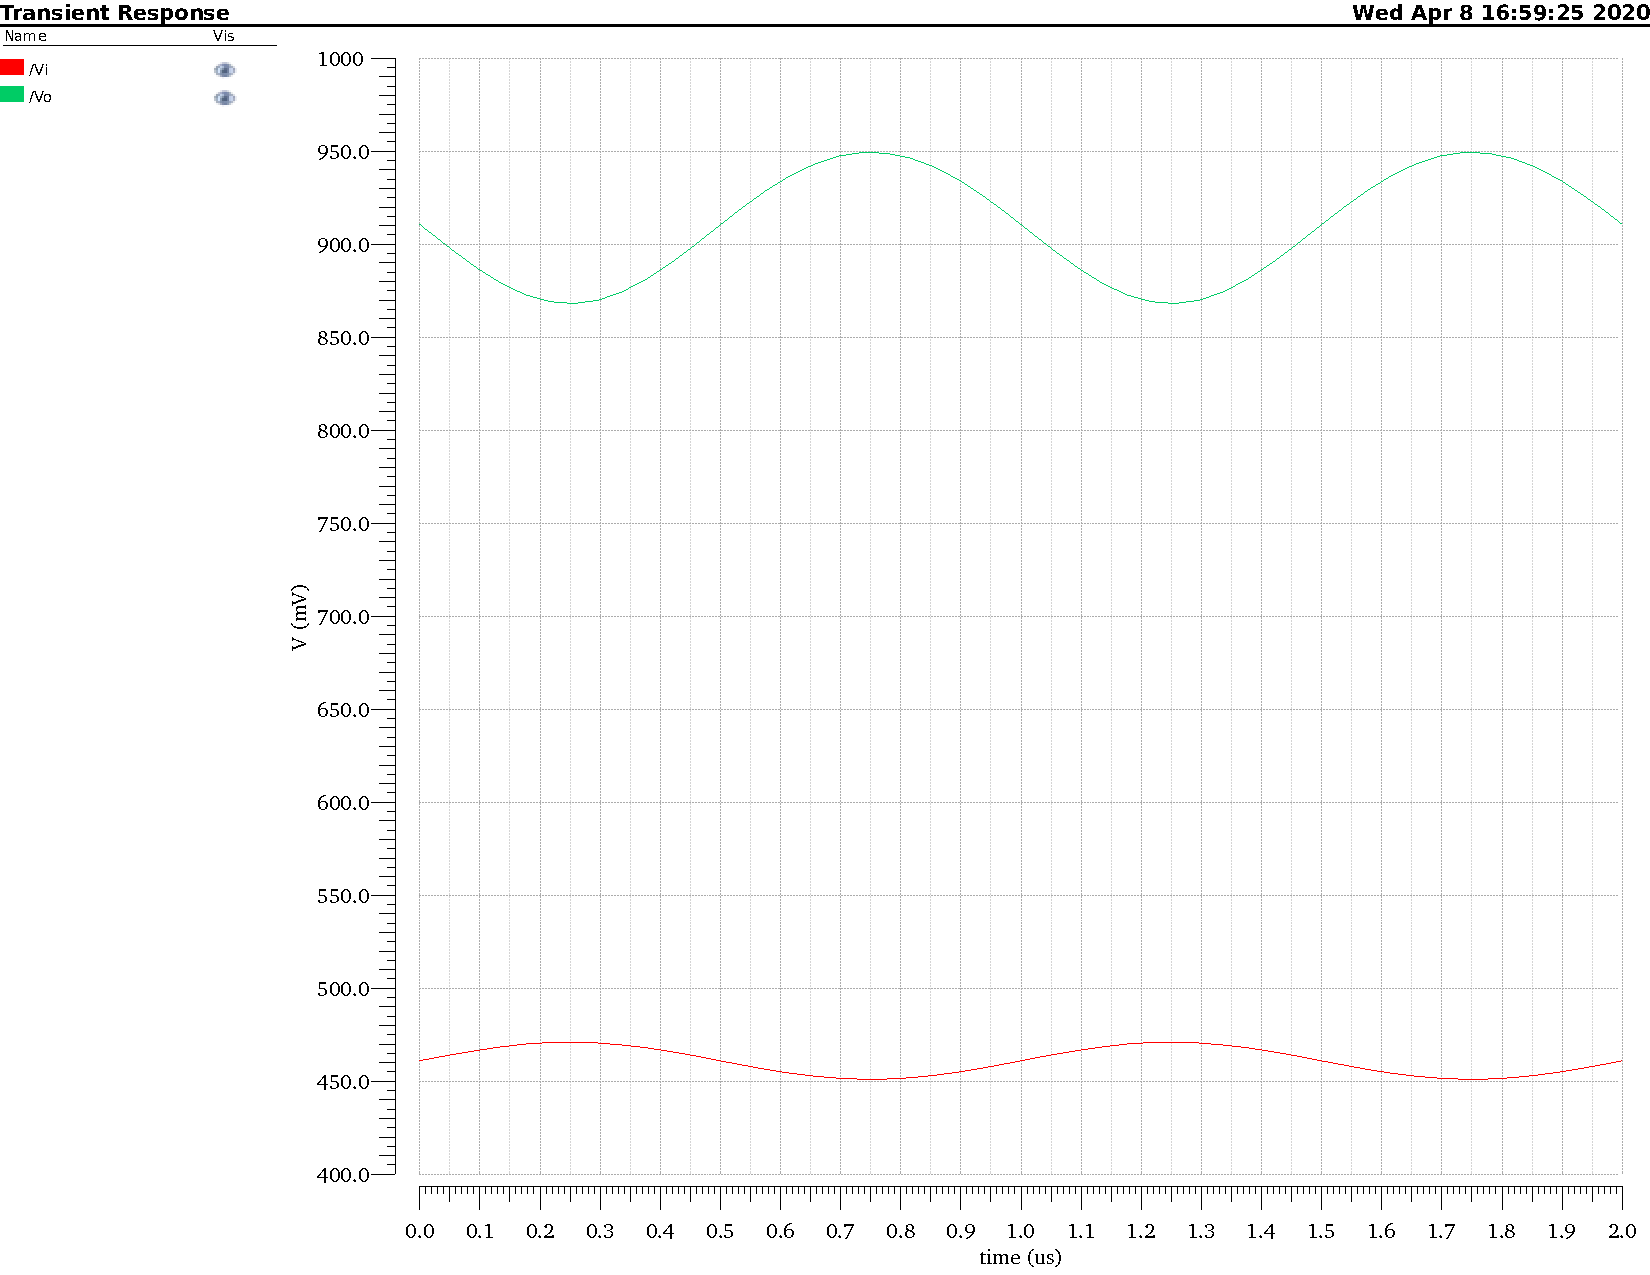
\includegraphics[width=\linewidth,page=1]{hw5}
		\includegraphics[width=\linewidth,page=2]{hw5}
	\end{center}
\end{document}